\documentclass{article}

% packages
\usepackage{amsmath, amsthm, thmtools, amsfonts, amssymb, luacode, catchfile, tikzducks, hyperref, ifthen}
\ifcsname c@kobocompile\endcsname
	\usepackage[a5paper, total={1072pt, 1448pt}, margin=10pt, includeheadfoot]{geometry} % set page margins
\else
	\usepackage[a4paper, margin=50pt, includeheadfoot]{geometry}
\fi
\usepackage[shortlabels]{enumitem}
\usepackage[skip=3pt, indent=0pt]{parskip}

% language
\usepackage[bidi=basic, layout=tabular, provide=*]{babel}
\ifcsname c@english\endcsname
	\babelprovide[main, import]{english}
\else
	\babelprovide[main, import]{hebrew}
	\babelprovide{rl}
\fi
%\babelfont{rm}{Libertinus Serif}
\babelfont{rm}[Renderer=Harfbuzz]{Libertinus Serif}
\babelfont{sf}{Libertinus Sans}
\babelfont{tt}{Libertinus Mono}

% style
\AddToHook{cmd/section/before}{\clearpage}	% Add line break before section
\linespread{1.3}
\setcounter{secnumdepth}{0}		% Remove default number tags from sections, this won't do well with theorems
\AtBeginDocument{\setlength{\belowdisplayskip}{3pt}}
\AtBeginDocument{\setlength{\abovedisplayskip}{3pt}}
\graphicspath{ {../images/} }

% operators
\DeclareMathOperator\cis{cis}
\DeclareMathOperator\Sp{Sp}
\DeclareMathOperator\tr{tr}
\DeclareMathOperator\im{Im}
\DeclareMathOperator\re{Re}
\DeclareMathOperator\diag{diag}
\DeclareMathOperator*\lowlim{\underline{lim}}
\DeclareMathOperator*\uplim{\overline{lim}}
\DeclareMathOperator\rng{rng}
\DeclareMathOperator\Sym{Sym}
\DeclareMathOperator\Arg{Arg}
\DeclareMathOperator\Log{Log}
\DeclareMathOperator\dom{dom}
\DeclareMathOperator\supp{Supp}
\DeclareMathOperator\var{Var}
\DeclareMathOperator\cov{Cov}

% commands
%\renewcommand\qedsymbol{\textbf{מש''ל}}
%\renewcommand\qedsymbol{\fbox{\emoji{lizard}}}
\newcommand{\Aa}[0]{\mathcal{A}}
\newcommand{\Bb}[0]{\mathcal{B}}
\newcommand{\CC}[0]{\mathbb{C}}
\newcommand{\Cc}[0]{\mathcal{C}}
\newcommand{\EE}[0]{\mathbb{E}}
\newcommand{\FF}[0]{\mathbb{F}}
\newcommand{\Ff}[0]{\mathcal{F}}
\newcommand{\Ii}[0]{\mathcal{I}}
\newcommand{\Gg}[0]{\mathcal{G}}
\newcommand{\Ll}[0]{\mathcal{L}}
\newcommand{\Mm}[0]{\mathcal{M}}
\newcommand{\NN}[0]{\mathbb{N}}
\newcommand{\Nn}[0]{\mathcal{N}}
\newcommand{\PP}[0]{\mathbb{P}}
\newcommand{\Pp}[0]{\mathcal{P}}
\newcommand{\QQ}[0]{\mathbb{Q}}
\newcommand{\RR}[0]{\mathbb{R}}
\newcommand{\Rr}[0]{\mathcal{R}}
\newcommand{\Ss}[0]{\mathcal{S}}
\newcommand{\TT}[0]{\mathbb{T}}
\newcommand{\Uu}[0]{\mathcal{U}}
\newcommand{\Vv}[0]{\mathcal{V}}
\newcommand{\Ww}[0]{\mathcal{W}}
\newcommand{\ZZ}[0]{\mathbb{Z}}
\newcommand{\acts}[0]{\circlearrowright}
\newcommand{\explain}[2] {
	\begin{flalign*}
		 && \text{#2} && \text{#1}
	\end{flalign*}
}
\newcommand{\maketitleprint}[0]{ \begin{center}
	%\begin{tikzpicture}[scale=3]
	%	\duck[graduate=gray!20!black, tassel=red!70!black]
	%\end{tikzpicture}	
	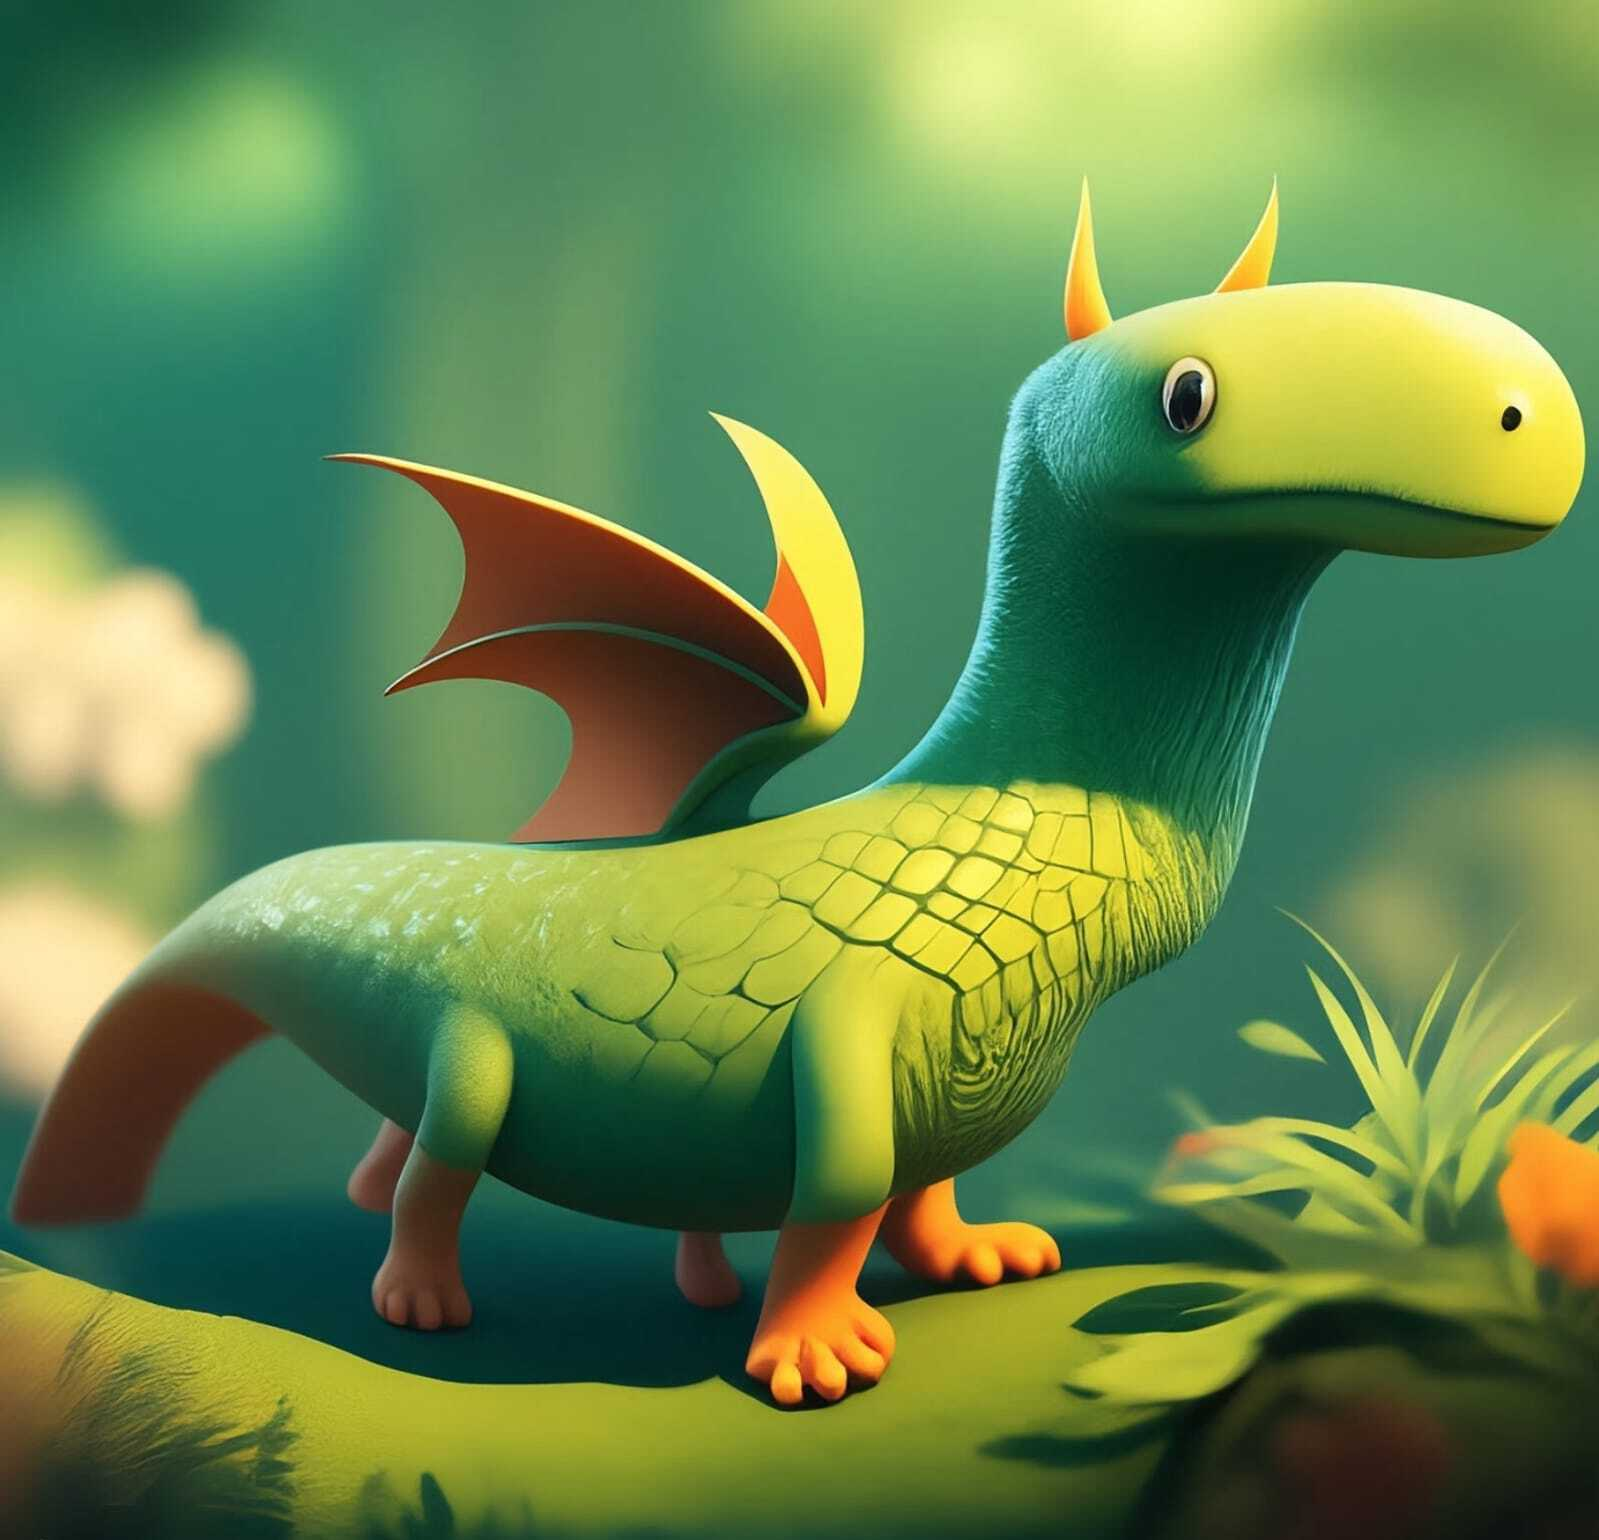
\includegraphics[width=6cm]{cover}
\end{center}
}

% theorem commands
\newtheoremstyle{c_remark}
	{}	% Space above
	{}	% Space below
	{}% Body font
	{}	% Indent amount
	{\bfseries}	% Theorem head font
	{}	% Punctuation after theorem head
	{.5em}	% Space after theorem head
	{\thmname{#1}\thmnumber{ #2}\thmnote{ \normalfont{\text{(#3)}}}}	% head content
\newtheoremstyle{c_definition}
	{3pt}	% Space above
	{3pt}	% Space below
	{}% Body font
	{}	% Indent amount
	{\bfseries}	% Theorem head font
	{}	% Punctuation after theorem head
	{.5em}	% Space after theorem head
	{\thmname{#1}\thmnumber{ #2}\thmnote{ \normalfont{\text{(#3)}}}}	% head content
\newtheoremstyle{c_plain}
	{3pt}	% Space above
	{3pt}	% Space below
	{\itshape}% Body font
	{}	% Indent amount
	{\bfseries}	% Theorem head font
	{}	% Punctuation after theorem head
	{.5em}	% Space after theorem head
	{\thmname{#1}\thmnumber{ #2}\thmnote{ \text{(#3)}}}	% head content

\ifcsname c@english\endcsname
	\theoremstyle{plain}
	\newtheorem{theorem}{Theorem}[section]
	\newtheorem{lemma}[theorem]{Lemma}
	\newtheorem{proposition}[theorem]{Proposition}
	\newtheorem*{proposition*}{Proposition}
	%\newtheorem{corollary}[theorem]{אין חלופה עברית}

	\theoremstyle{definition}
	\newtheorem{definition}[theorem]{Definition}
	\newtheorem*{definition*}{Definition}
	\newtheorem{example}{Example}[section]
	\newtheorem{exercise}{Exercise}[section]

	\theoremstyle{remark}
	\newtheorem*{remark}{Remark}
	\newtheorem*{solution}{Solution}
	\newtheorem{conclusion}[theorem]{Conclusion}
	\newtheorem{notation}[theorem]{Notation}
\else
	\theoremstyle{c_plain}
	\newtheorem{theorem}{משפט}[section]
	\newtheorem{lemma}[theorem]{למה}
	\newtheorem{proposition}[theorem]{טענה}
	\newtheorem*{proposition*}{טענה}
	%\newtheorem{corollary}[theorem]{אין חלופה עברית}

	\theoremstyle{c_definition}
	\newtheorem{definition}[theorem]{הגדרה}
	\newtheorem*{definition*}{הגדרה}
	\newtheorem{example}{דוגמה}[section]
	\newtheorem{exercise}{תרגיל}[section]

	\theoremstyle{c_remark}
	\newtheorem*{remark}{הערה}
	\newtheorem*{solution}{פתרון}
	\newtheorem{conclusion}[theorem]{מסקנה}
	\newtheorem{notation}[theorem]{סימון}
\fi

% Questions related commands
\newcounter{question}
\setcounter{question}{1}
\newcounter{sub_question}
\setcounter{sub_question}{1}

\ifcsname c@english\endcsname
	\newcommand{\question}[1][0]{
		\ifthenelse{#1 = 0}{}{\setcounter{question}{#1}}
		\section{Question \arabic{question}}
		\addtocounter{question}{1}
		\setcounter{sub_question}{1}
	}

	\newcommand{\subquestion}[1][0]{
		\ifthenelse{#1 = 0}{}{\setcounter{sub_question}{#1}}
		\subsection{Part \alph{sub_question}}
		\addtocounter{sub_question}{1}
	}
\else
	\newcommand{\question}[1][0]{
		\ifthenelse{#1 = 0}{}{\setcounter{question}{#1}}
		\section{שאלה \arabic{question}}
		\addtocounter{question}{1}
		\setcounter{sub_question}{1}
	}

	\newcommand{\subquestion}[1][0]{
		\ifthenelse{#1 = 0}{}{\setcounter{sub_question}{#1}}
		\subsection{סעיף \localecounter{letters.gershayim}{sub_question}}
		\addtocounter{sub_question}{1}
	}
\fi

% import lua and start of document
\directlua{common = require ('../common')}

\GetEnv{AUTHOR}

% headers
\author{\AUTHOR}
\date\today

\title{פתרון מטלה 06 --- מבוא לטופולוגיה, 80516}
% chktex-file 9
% chktex-file 17

\begin{document}
\maketitle
\maketitleprint[purple]

\question[2]
\subquestion{}
יהיו מרחבים טופולוגיים $X, Y$ כך ש־$X$ קומפקטי ו־$Y$ האוסדורף.
נניח גם כי $f : X \to Y$ רציפה.
נראה ש־$f$ העתקה סגורה.
\begin{proof}
	נבחין כי $f(X)$ היא תת־קבוצה קומפקטית של $Y$.
	אם קיימים $y \in Y \setminus f(X)$ אז הם לא משפיעים על הרציפות של $f$ או על תכונת האוסדורף, לכן נניח ללא הגבלת הכלליות ש־$Y = f(X)$.
	נניח ש־$C \subseteq X$ סגורה, אז היא קומפקטית, לכן גם $f(C)$ קומפקטית, וכן $f(C)$ האוסדורף, ולכן גם סגורה.
\end{proof}

\subquestion{}
יהיו מרחבים טופולוגיים $X, Y$ כך ש־$X$ קומפקטי ו־$Y$ האוסדורף.
נניח ש־$f : X \to Y$ היא רציפה וחד־חד ערכית.
נראה ש־$f$ היא הומיאומורפיזם בין $X$ והתמונה $f(X) \subseteq Y$.
\begin{proof}
	כמו בסעיף הקודם מטעמי פשטות נניח ש־$Y = f(X)$, נוכל אחרת להגדיר $Y' = f(X)$ וההוכחה תישאר זהה.
	נובע אם כך ש־$f$ חד־חד ערכית ועל $Y$, ורציפה.
	אז נובע ממשפט מההרצאה שאכן $f$ הומיאומורפיזם.
\end{proof}

\question{}
בשאלה זו נדון בקבוצת קנטור.
נגדיר את $C$ להיות קבוצת קנטור.

\subquestion[2]
נגדיר את הפונקציה $f : {\{0, 1\}}^\NN \to C$ על־ידי,
\[
	f(s)
	= \sum_{n = 0}^\infty \frac{2 s_n}{3^{n + 1}}
\]
נוכיח ש־$f$ חד־חד ערכית ועל.
\begin{proof}
	נזכור שהגדרנו את $C = \bigcap_{n = 0}^\infty C_n$ עבור $C_{n + 1} = \frac{1}{3} C_n \cup (\frac{2}{3} + \frac{1}{3} C_n)$,
	וכן אנו יודעים כי $x \in C_n$ אם ורק אם אפשר לכתוב אותו בפיתוח טרינרי ללא הספרה $1$ ב־$n$ הספרות הראשונות.

	נראה חד־חד ערכיות.
	נניח ש־$s, s' : \NN \to \{0, 1\}$ כך ש־$s \ne s'$, ונניח ש־$m \in \NN$ מעיד על כך, כלומר $s(m) \ne s'(m)$.
	נניח גם ללא הגבלת הכלליות ש־$s(m) = 0 < 1 = s'(m)$.
	אז מהגדרת $f$ נקבל ש־$f(s') - f(s) \ge \frac{1}{3^{m + 1}}$, כאשר אי־השוויון נקבע בשל הייצוג הטרינרי של המספרים ואי־יחידות הייצוג.
	נסיק מאי־השוויון שבפרט $f(s) \ne f'(s)$.

	נבדוק על.
	נניח ש־$x \in C$ ונניח ש־$x = 0.x_1 x_2 \ldots$ ייצוג טרינרי, כלומר $x_i \in \{0, 1, 2\}$ לכל $i \in \NN$.
	נגדיר $s : \{0, 1\} \to \NN$ על־ידי $s(n) = \frac{x_n}{2}$ לכל $n$.
	נבחין כי כמסקנה מהעובדה $x_i \in \{0, 2\}$ בלבד, ולכן גם $\frac{x_i}{2} \in \{0, 1\}$ בלבד.
	מהגדרת הייצוג הטרינרי והגדרת $f$, מתקיים $f(s) = 0.x_1 x_2 \ldots = x$ כפי שרצינו.
\end{proof}

\subquestion{}
נראה ש־$f$ הומיאומורפיזם ממרחב מהכפלה ${\{0, 1\}}^\NN$ עם טופולוגיית מכפלה מעל טופולוגיה דיסקרטית.
\begin{proof}
	נראה ש־$f^{-1} : C \to {\{0, 1\}}^\NN$ רציפה.
	נניח ש־$U \subseteq {\{0, 1\}}^\NN$ פתוחה, ונניח ש־$m$ אינדקס שאחריו $U_n = \{0, 1\}$ לכל $n > m$.
	כלומר לכל $x \in {(f^{-1})}^{-1}(U) = f(U)$ נסיק ש־$B_{\frac{1}{3^m}}(x) \subseteq f(U)$.
	זהו כמובן איחוד סופי של קבוצות פתוחות ולכן נסיק ש־$f(U)$ פתוחה, ולכן $f^{-1}$ רציפה.

	נבחין כי $C = \bigcap_{n = 0}^\infty C_n$ עבור $C_n \subseteq [0, 1]$ סגורה ולכן $C$ סגורה וחסומה ולכן קומפקטית.
	נבחין גם כי טופולוגיה דיסקרטית תמיד גוררת האוסדורף, וכן מכפלת מרחבים משמרת תכונת האוסדורף, ולכן ${\{0, 1\}}^\NN$ מרחב האוסדורף.
	נסיק על־ידי שאלה 2 סעיף ב' ש־$f$ הומיאומורפיזם.
\end{proof}

\subquestion{}
נוכיח שקבוצת קנטור היא בלתי קשירה לחלוטין, דהינו רכיבי הקשירות שלה הם יחידונים.
\begin{proof}
	ראינו בהרצאה שאם $f$ רציפה אז תמונת קבוצה קשירה היא קשירה, נרחיב את הטענה לשני הכיוונים ונקבל שקבוצה $U \subseteq {\{0, 1\}}^\NN$ היא קשירה אם ורק אם $f(U) \subseteq C$ קשיר. \\
	אם כך מספיק להראות שכל יחידון הוא רכיב קשירות ב־${\{0, 1\}}^\NN$.
	יהי $s : \NN \to \{0, 1\}$, ותהי $U \subseteq s$ סביבה פתוחה שלו.
	אז נבחר את הצמצום $U_1 = U \cap \{ f : \NN \to \{0, 1\} \mid f(m) = s(m) \}$ ל־$m$ שרירותי כך ש־$U_1 \subsetneq U$.
	לכן נוכל להסיק ש־$U$ לא קשיר ובפרט לא רכיב קשירות של $s$.
	נסיק שרכיב הקשירות $U$ של $s$ מקיים $\forall f \in U, \forall n \in \NN,\ f(n) = s(n)$, ובהכרח $U = \{ s \}$.
\end{proof}

\question{}
\subquestion{}
נראה ש־$\RR$ קומפקטי מקומית.
\begin{proof}
	תהי $x \in \RR$, אז נבחר $C_x = [x - 1, x + 1]$, נבחין כי $x \in (x - 1, x + 1) \subseteq C_x$, כלומר זוהי קבוצה סגורה המכילה סביבה פתוחה של $x$.
	אנו יודעים כי $\RR$ מרחב מטרי, ולכן קומפקטיות שקולה במרחב זה לסגירות וחסימות, ואכן $C_x$ חסומה וסגורה, ולכן קומפקטית.
\end{proof}

\subquestion{}
בכל תת־סעיף נגדיר מרחב ונראה שהוא לא קומפקטי מקומית.

\subsubsection{i}
נבחן את $\QQ$ עם הטופולוגיה הסטנדרטית.
\begin{proof}
	נראה ש־$\QQ$ לא קומפקטי מקומית בסביבת $q$.
	נניח ש־$q \in U \subseteq K$ עבור $U$ פתוחה ו־$K$ קומפקטית.
	$K$ קומפקטית במרחב מטרי ולכן גם קומפקטי סדרתית.
	יהי $a \in \RR \setminus \QQ$ כך ש־$a$ פנימי לקטע $\overline{K}$ מעל הממשיים, ונגדיר איזושהי סדרת נקודות ${\{ q_n \}}_{n = 1}^\infty \subseteq K$ כך ש־$q_n \to a$.
	נקבל ש־$a \in K$ בסתירה ל־$a \notin \QQ$.
\end{proof}

\end{document}
